\documentclass[12pt]{article}

\usepackage{amsmath}
\usepackage[utf8]{inputenc}
\usepackage[T1]{fontenc}
\usepackage[magyar]{babel}
\usepackage{graphicx}
\usepackage{float}
\usepackage[paper=a4paper,margin=1in]{geometry}

\usepackage{siunitx}
%%\title{%
%%  Kondenzált anyagok fizikája \\
%%  \large 1. Gyakorlat}
%%\author{}  
%%\maketitle


\begin{document}


\centerline{
\textsc{\Large{ Kondenzált anyagok fizikája}}
}
\centerline{ 
\textsc{\large{1. Gyakorlat}}
}
\vspace{10mm}
\textbf{Gy1.} Hány féle rács lehetséges 2D-ban? (Segítség: $a$, $b$ és $\alpha$  cellaparaméterek)
\\

\textbf{Gy2.} Milyen a Bravais-rács és hány atom van az elemi cellában az ábrán látható Kagomé-rács, illetve gyémántszerkezet esetén?

\begin{figure}[h!]

\begin{center}


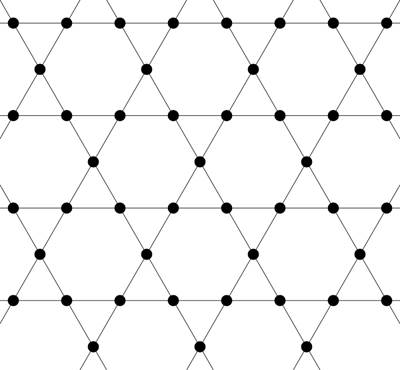
\includegraphics[height=4cm]{KagomeLattice.jpg} \hspace{10mm}
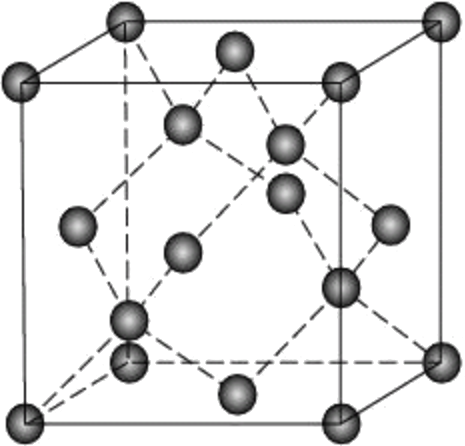
\includegraphics[height=4cm]{gyemant.png}
\end{center}
\end{figure}

\textbf{Gy3.} Az alábbi Escher-grafika gekkók kétdimenziós rácsát ábrázolja. Állapítsuk meg a Bravais-rácsot és rajzoljunk be egy primitív elemi cellát! Hány gekkó van az elemi cellában?
\begin{figure}[h!]
\begin{center}
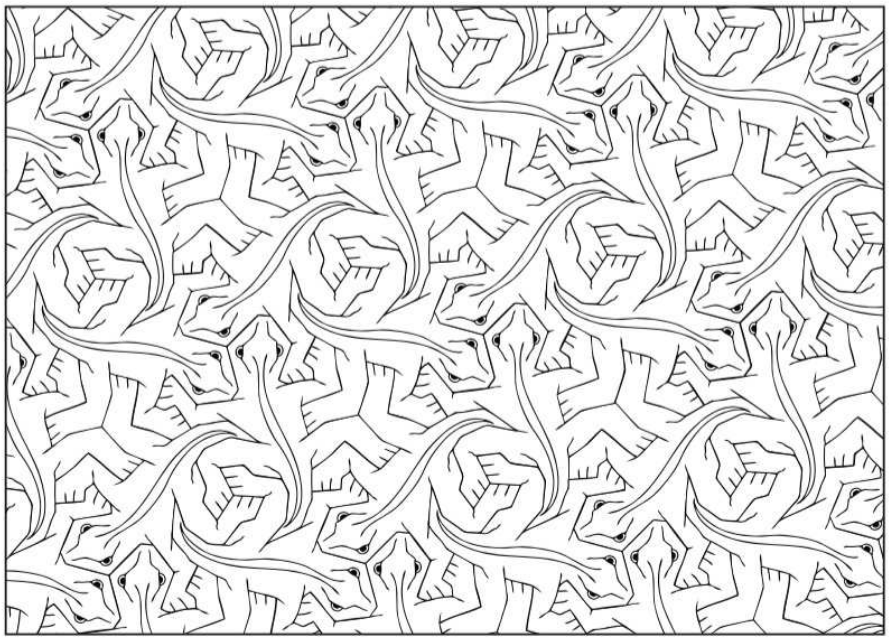
\includegraphics[height=5cm]{../../abrak/1-Escher.png}
\end{center}
\end{figure}

\textbf{Gy4.} Mutassuk meg, hogy 
a) a lapon centrált kockarács (FCC) reciprokrácsa testcentrált kockarács (BCC);
b) a testcentrált kockarács (BCC) reciprokrácsa lapon centrált kockarács (FCC)
\\

\textbf{Gy5.} Adjuk  meg  az  elemi  rácsvektorokat kétdimenziós  szabályos háromszögrács esetén,  valamint  a  rácsvektorok  által  meghatározott  elemi  cellát  és  a Wigner-Seitz  cellát.  Adjuk  meg  a reciprokrács elemi rácsvektorait. Milyen rácsot határoznak meg? Számoljuk ki a direkt rács és a reciprokrács Wigner-Seitz cellájának területét.
\\

\textbf{Gy6.} Egy kristályrács primitív rácsvektorait egy derékszögű koordinátarendszerben az (1, 2, 1), (0, 0, 2), (1, 0, -1) számhármasok reprezentálják, ahol mindent $\si{\angstrom}$ngströmben mérünk. Adjuk meg a reciprokrács primitív rácsvektorait reprezentáló számhármasokat $\si{\angstrom}^{-1}$ egységekben




\end{document}